\chapter{Testing and Analysis}
\label{sec:results}

With a theoretical proof of our algorithm complete, we can move on to
testing and analyzing its real-world tractability and performance. We want to
confirm that the time synchronization protocol is able to give accurate clock
uncertainty bounds to provide overlapping freeze windows. We also
want to test and analyze the size of these freeze windows in practice
to ensure that they are not too large causing implementation infeasible.

FIGURE OUT EXPLAINING NTP AND WHY WE CHOSE NTP SO WE NOW WE CHOSE NTP

This chapter is split into two sections. The first section includes
the setup of the simulation environment for NTP and its parameters,
and data collection of those parameters on a live Ceph test cluster.
The second section consists of the results and analyses from the simulations,
including the correctness of the NTP uncertainty bounds and the implied
performance from the size of the freeze windows.

ADD RESULTS?



\section{Collection of NTP Performance in a Real-World Setting}

There are two primary characteristics of our algorithm that need
testing: the existence of the freeze period overlaps, and the 
worst and average case duration of these freeze periods. 
The existence of the freeze period overlaps can be tested by 
ensuring that all of the NTP uncertainty bounds overlap at some 
point in time. Since individual nodes cannot know the real time
(if it did, we would be done as there would be no need for clock uncertainty
bounds), we must use simulations to observe the existence of 
the overlap of freeze windows. In order to accurately simulate the
characteristics of a real Ceph cluster, we need to model the
behavior of a live Ceph cluster.

To test on a live Ceph cluster, we need to log data on 
instances of NTP running on the cluster. The implementation for NTP 
used on the Ceph cluster is called \textit{ntpd}. \textit{ntpd} is a
daemon that synchronizes the clocks on each machine using NTP and
provides diagnostic data on the machines' clocks and network 
communications. The two parameters of interest are frequency offset and
network latency. The \textit{ntpd} daemons were running on a Ceph
test cluster that include three types of computers named Mira,
Plana, and Burnupi. Miras and Planas use Intel-based chips, while
Burnupi uses AMD chips.

The frequency offset is the estimated random error on a given computer's
clock drift from the NTP server, and is typically measured in Parts
Per Million (PPM). For example, a PPM of 10 for frequency offset would
mean for every million clock ticks of the NTP server, the local
computer could be off by 10 ticks. The network latency is a measure of
the round trip time of the message passed between a local machine in
the Ceph cluster to the NTP server and back. The round trip time
is typically on the order of milliseconds~\cite{Sage}.


The histogram in Figure~\ref{fig:latency-hist} shows the logged
values of network latency in the cluster. The mean is 2.668 ms, the 
standard deviation is 10.304 ms, and the median is 0.643 ms. The 
difference in network latency between each type of machine is not
statistically significant, as we would expect given that the network
latency between machines should not depend on the types of 
machines in the network. 

\begin{figure}[h]
  \centering
  \caption{~Histogram of network latency across 234 nodes in a Ceph test cluster.} 
  \label{fig:latency-hist}
  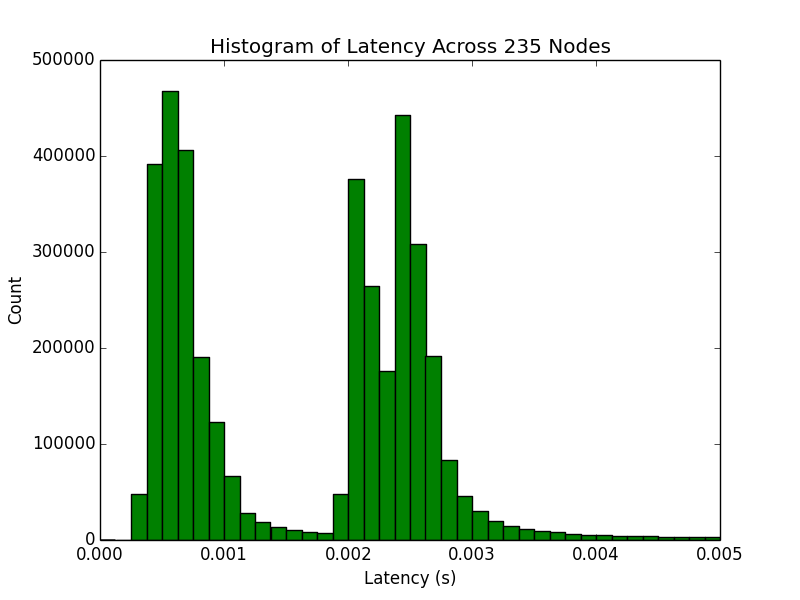
\includegraphics[width=0.8\textwidth]{latency-hist.png}
\end{figure}

Figure~\ref{fig:burnupi-hist}, Figure~\ref{fig:mira-hist},
and Figure~\ref{fig:plana-hist} show the behavior of clock frequency offset
on the three types of machines in the Ceph cluster. Despite the different offsets, 
these are consistent with a normal distribution. These values are reasonable 
as we would generally expect frequency offset to be at most $\pm 20$ PPM. 
The average frequency offset for individual Burnupi machines is -5.216 PPM with 
average standard deviation 1.079 PPM, Mira nodes with 10.752 PPM with average
standard deviation 0.356, and Plana nodes with 13.341 PPM with average standard deviation 1.690. The average standard deviation across all nodes is
1.033 PPM. It is interesting to note that the Burnupi machines with 
the AMD chips primarily negative clock frequency offset, while the 
Mira and Plana machines with Intel chips have primarily positive 
clock frequency offsets.

\begin{figure}[h]
  \centering
  \caption{~Histogram of NTP's frequency offset for Burnupi machines in the Ceph test cluster.}
  \label{fig:burnupi-hist}
  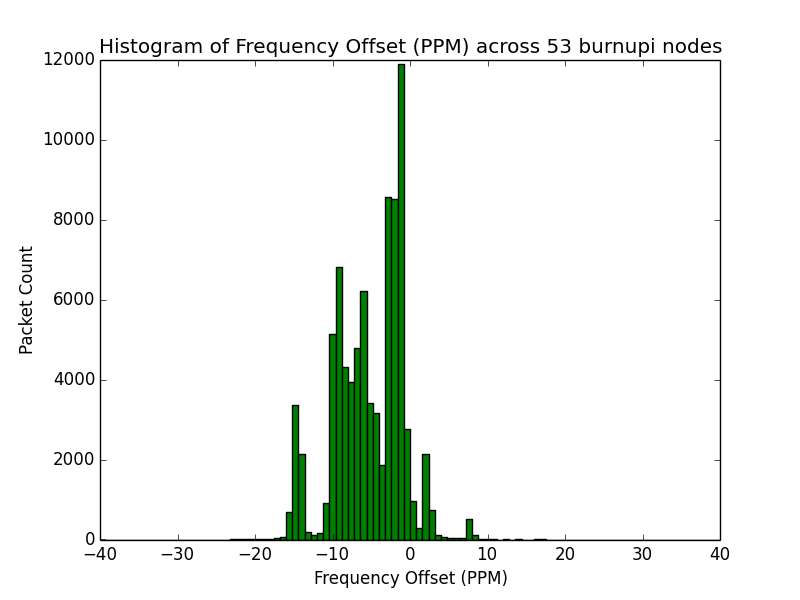
\includegraphics[width=0.8\textwidth]{burnupi-freq-offset.png}
\end{figure}

\begin{figure}[h]
  \centering
  \caption{~Histogram of NTP's frequency offset for Mira machines in the Ceph test cluster.}
  \label{fig:mira-hist}
  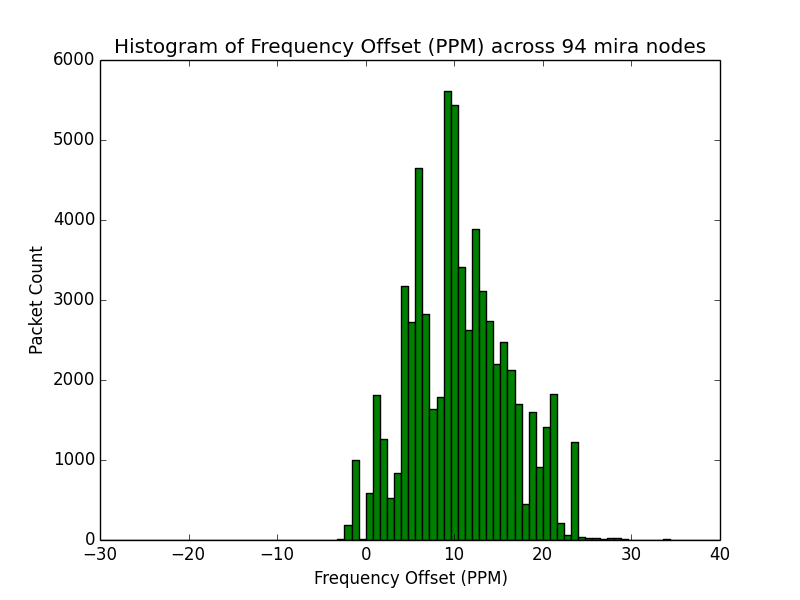
\includegraphics[width=0.8\textwidth]{mira-freq-offset.png}
\end{figure}

\begin{figure}[h]
  \centering
  \caption{~Histogram of NTP's frequency offset for Plana machines in the Ceph test cluster.}
  \label{fig:plana-hist}
  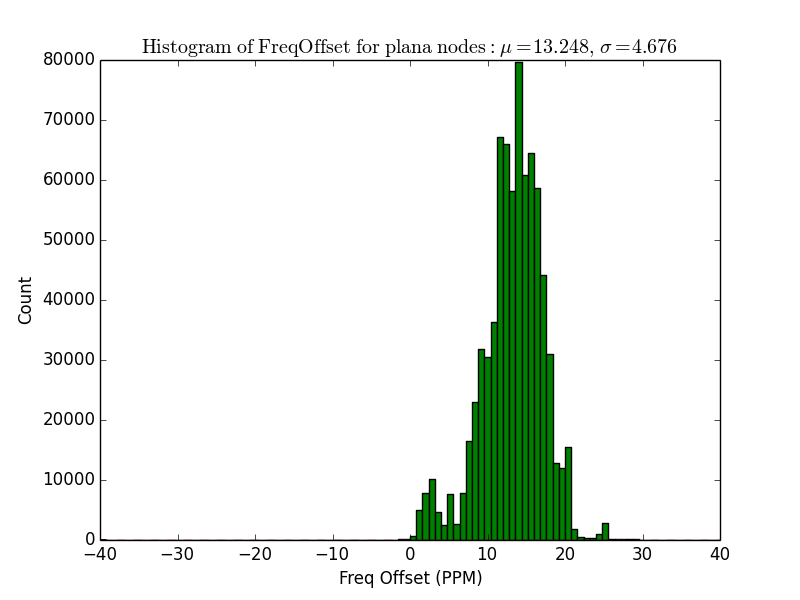
\includegraphics[width=0.8\textwidth]{plana-freq-offset.png}
\end{figure}

With the data collected on frequency offset and network latency, we can 
now simulate a test cluster with input parameters that reflect the 
real world. Recall the fact that we cannot simply use a real Ceph
cluster to observe the overlapping freeze windows because there is no
way on observing the real time on a given computer. A
simulated network environment running on a single computer has the
advantage of having a single clock on which all simulated clocks are
based. By having a single clock, we are able to quantify and verify
the claims that time synchronization algorithms make about the quality
of a synchronization and the quality of the clocks involved.

% NOTE: I'm not sure this paragraph is needed?
% By using a simulation that abstracts the clock from a physical clock,
% we also eliminate any potential for idiosyncrasies of the host system
% clock to affect the measurements gathered in the simulation. This has
% the added benefit of allowing the simulation to run at a speed much
% greater than real time.

We have chosen to use an environment called \textit{clknetsim} %% TODO reference to clknetsim repo?
to conduct our simulations. \textit{Clknetsim} is an open-source simulation 
package developed and used by a major contributor to the \textit{Chrony}
project <TODO citation> and the \textit{linuxptp} project <TODO citation> 
to test these protocol implementations. In
comparison to commercial network simulation products, it provides a 
simple codebase and feature set targeted at measuring 
time across a simulated network. We have made slight additions to and
modifications of the clknetsim package. These extensions were made in 
order to expose state parameters of NTP that were not being exposed, 
including the maximum error term.

Clknetsim makes use of the environment variable \textit{LD\_PRELOAD} in
the Linux library to intercept system calls that time sychronization 
libraries make on their hosts. Using these intercepted calls, 
clknetsim is able to monitor and capture the internal state of
the synchronization program. It is also able to fully control the
information the host's time library receives from the network and the system
clock. As clknetsim is manipulating system clocks and network
connections for the simulation, it can shape the behavior of the clock
and network parameters to test different setups and hardware properties. 
        
We are most interested in measuring two parameters in
this system. We first want to determine if the maximum uncertainty
reported by NTP is accurate. We can check that the maximum uncertainty
report is accurate by ensuring that the uncertainty bounds on a given machine
clock's time includes the real time.
Clknetsim allows us to do this by, for a
given timestamp in the simulation, allowing us to observe what NTP
thinks the time is along with information about how certain NTP is
about that time. Our second goal is to analyze how low of an
uncertainty can be reached. As our algorithm is predicated on a upper
bound of the uncertainty in time, performance analysis can be
accomplished by observing how modifying various parameters such as
network latency affect the maximum error term that NTP reports.


